\documentclass[a4paper]{article}
\usepackage[utf8]{inputenc}
\usepackage[francais]{babel}
\usepackage[babel=true]{csquotes}
\usepackage{graphicx}
\usepackage{listings}
\usepackage{fullpage}

\pagestyle{headings}

\title{Programming techniques : Project 2}
\author{Marien Bourguignon, Ramzi Mhadhbi \& Raphaël Javaux}
\date{}

\begin{document}

\maketitle

    \paragraph{} We implemented four different symbol table data structures and
measured the time and memory usage for each structure in various conditions.
Each of our symbol table stores 32 bits integer keys.

\section{Data structures comparison}

\subsection{BST}

    \paragraph{} Our Binary Search Tree is our simplest symbol table. While its
average complexity for item insertion and item lookup is pretty good by being
quasiconstant $O(log(n))$\footnote{Each time complexity is computed on the
number of comparisons.}, its linear $O(n)$ worst case complexity is really
harmful on large inputs.

\subsection{RBT}

    \paragraph{} Our Red Black Tree removes the worst case complexity of the
BST (which is $O(log(n))$). But its operations are more complex and so this
structure is a little bit slower on best cases that a BST.

\subsection{TST}

    \paragraph{} Our Ternary Search Tree encodes the integer keys as strings.
This limits the depth of the tree to the maximum length of a character encoded
32 bits integer (which is constant). So the average and worst case of this 
structure is $O(1)$. But encoding an integer as a string is a relatively slow 
operation and requires a lot of space.

\subsection{Hash table with linear probing}

    \paragraph{} We implemented a self-resizing hash table. The hash-table
internal vector starts with a size of 8 cells and doubles its size every time
the total number of occupied cells exceeds 50\% of its size, to avoid
collisions.
Hash tables are very fast and provides a constant complexity ($O(1)$) for lookup 
and insertion if collisions are mostly avoided.
\newline
Hash tables complexity doesn't change with the order the item are inserted.

\section{Time measurements}

    \paragraph{} We measured our structures with three different types of
inputs (which differ by the order of the insertions) :

\subsection{Ascending and descending ordered integers}

    \paragraph{} BST are inefficient when data are inserted in order because the
tree looks like a singly linked list. Each insertion requires to traverse the 
entire structure. Especially, hash tables are way faster, probably because the lower complexity
and cache efficiency.
The following graph shows how the insertion time grows rapidly with the BST when
the number of items grows (horizontal values) :

    \begin{center}
        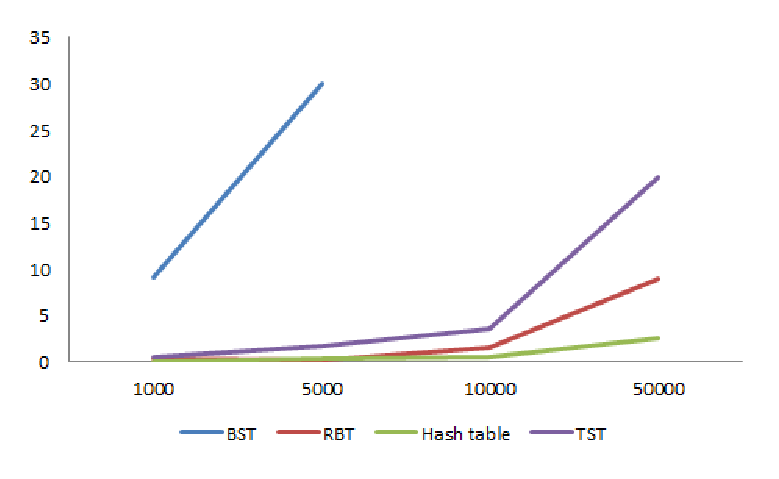
\includegraphics[width=270pt]{insertions_enordre.eps}
    \end{center}

The graph is similar for searches. Tries are a little bit faster when we are 
looking at existing items instead of keys which are not in the symbol table.

\subsection{Randomly ordered integers}

    \paragraph{} The BST is quite efficient on the insertion of perfectly 
random input, but the hash table is still the fastest symbol table:

    \begin{center}
        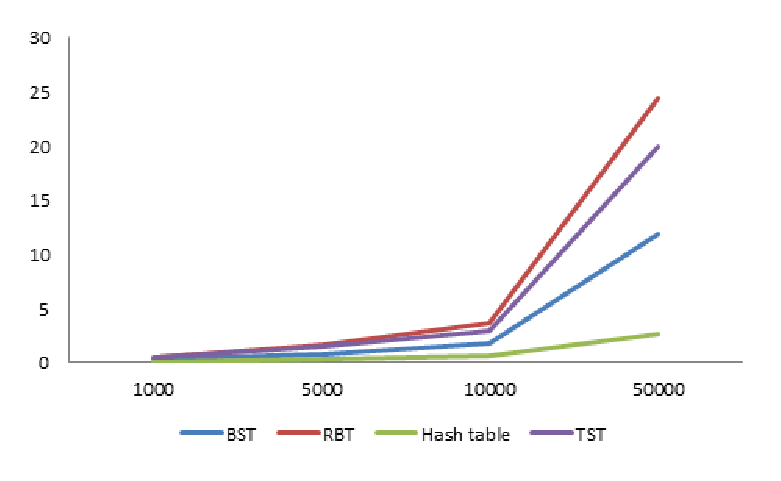
\includegraphics[width=270pt]{insertions_random.eps}
    \end{center}

This is because the BST is the simplest tree and random data is not far away
for the best use case of the structure. As predicted, hash tables speed don't
change with the way data are inserted.

\section{Memory measurements}

    \paragraph{} The space usage is directly computable from the number of 
inserted item.

    \paragraph{BST} Our BST uses the following C structure\footnote{item\_t is
the type of the stored items, in this case, 32 bits integers.}:
\begin{lstlisting}
typedef struct _bst_t {
    item_t item;
    struct _bst_t *left, *right;
} bst_t;
\end{lstlisting}
Each item requires a such structure to be allocated. This structure is 12 bytes
long\footnote{On an Intel 32 bits computer.}.

    \paragraph{RBT} Our RBT uses the following C structure:
\begin{lstlisting}
typedef struct _rbt_t {
    item_t item;
    struct _rbt_t *left, *right;
    bool red;
} rbt_t;
\end{lstlisting}
Each item requires a such structure to be allocated. This structure is 16 bytes
long.

    \paragraph{TST} Our TST uses the following C structure:
\begin{lstlisting}
typedef struct _tst_t {
    char value;
    struct _tst_t *left, *middle, *right;
} tst_t;
\end{lstlisting}
Each character of a key need to allocate a such structure (except a few for
the first levels of the tree). This structure is 16 bytes long and the average
key is 6 characters long. This is the most expensive structure.

    \paragraph{Hash table} Each cell of our hash table uses the following
C structure:
\begin{lstlisting}
typedef struct {
    bool used;
    item_t item;
} ht_cell_t;
\end{lstlisting}
If $n$ items has been inserted in the hash table, then at least $2n$ such 
structures has been allocated. This structure is 8 bytes long.

    \paragraph{} The following graph shows how these values grow :

    \begin{center}
        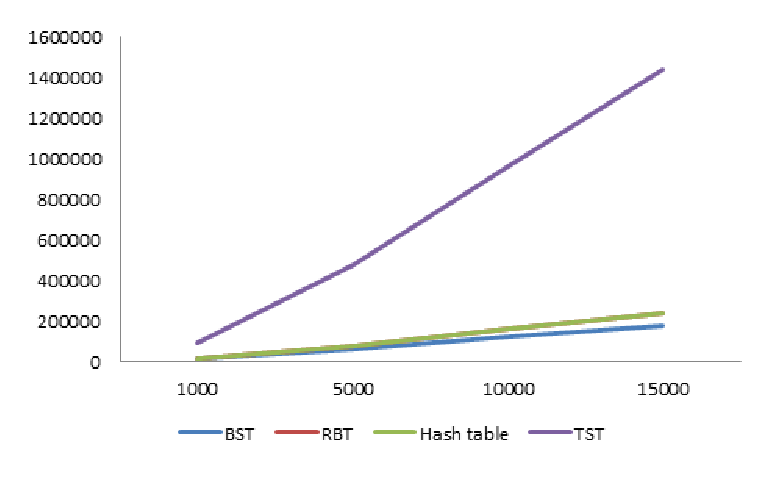
\includegraphics[width=270pt]{memory.eps}
    \end{center}

The BST uses a little bit less space than the hash table or the RBT (they use
more or less the same space). The TST uses a very large amount of space.

\section{Conclusion}

    \paragraph{}The project showed us that after choosing a data structure that
fits our needs, we also need to find the right implementation according to how
we are going to use it.

    \paragraph{} For example, a less naive implementation will probably have a 
lower running time for the same amount of data, but may uses more memory, which 
can also be problematic (depending of the kind of hardware we use).

\end{document}